\documentclass{standalone}
\usepackage[dvipsnames]{xcolor}
\usepackage{tikz}
\usetikzlibrary{positioning, calc, shapes, fit, backgrounds, patterns}

\begin{document}
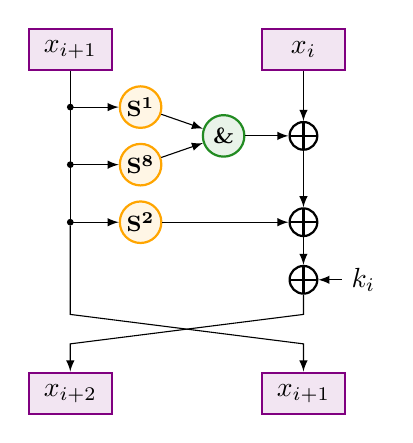
\begin{tikzpicture}
\tikzstyle{roundblock}=[draw=Purple, thick, fill=Purple!10, minimum width=30pt, minimum height=15pt]
\tikzstyle{function}=[draw=Orange, circle, thick, fill=Orange!10, minimum size=15pt,
font=\footnotesize\bfseries, node distance=5pt, inner sep=0pt]
\tikzstyle{XOR}=[draw,circle, minimum size=10pt, thick, append after command={
      [shorten >=\pgflinewidth, shorten <=\pgflinewidth,]
      (\tikzlastnode.north) edge[thick] (\tikzlastnode.south)
      (\tikzlastnode.east) edge[thick] (\tikzlastnode.west)},
    node distance=10pt]
\tikzstyle{junct}=[inner sep=0pt, circle, draw, fill=black, minimum size=2pt]

% inputs
\node (inpx) [roundblock] {$x_{i+1}$};
\node (inpy) [roundblock, right=of inpx, xshift=25pt] {$x_i$};

% shifts
\node (s1) [function, below=of inpx.south east, xshift=10pt] {S\textsuperscript{1}};
\node (s8) [function, below=of s1] {S\textsuperscript{8}};
\node (s2) [function, below=of s8] {S\textsuperscript{2}};

% and
\node (and) at ($(s1)!0.5!(s8)$) [function, draw=ForestGreen, fill=ForestGreen!10, xshift=30pt] {\&};

% xors
\node (xor1) at (and -| inpy) [XOR] {};
\node (xor2) at (s2 -| xor1) [XOR] {};
\node (xor3) [XOR, below=of xor2] {};

\node (key) [right=of xor3, xshift=-20pt] {$k_i$};

% connections
\draw[-latex] (s1) -- (and);
\draw[-latex] (s8) -- (and);
\draw[-latex] (and) -- (xor1);
\draw[-latex] (s2) -- (xor2);
\draw[-latex] (inpy) -- (xor1);
\draw[-latex] (xor1) -- (xor2);
\draw[-latex] (xor2) -- (xor3);
\draw[-latex] (inpx.south) |- node (junct1) [junct] {} (s1);
\draw[-latex] (junct1) |- node (junct2) [junct] {} (s8);
\draw[-latex] (junct2) |- node (junct3) [junct] {} (s2);
\draw[-latex] (key) -- (xor3);

% out
\node (outx) [roundblock,  below=of inpx, yshift=-80pt] {$x_{i+2}$};
\node (outy) [roundblock, right=of outx, xshift=25pt] {$x_{i+1}$};

\draw[-latex] (xor3.south) -- ++(0, -0.25) node (coord1) {} -- ([yshift=10pt]outx.north) -- (outx.north);
\draw[-latex] (junct3) -- (coord1 -| junct3) -- ([yshift=10pt]outy.north) -- (outy.north);


\end{tikzpicture}
\end{document}
